\documentclass[12pt, a4paper]{article}

% Packages
\usepackage[utf8]{inputenc}
\usepackage[T1]{fontenc}
\usepackage[spanish]{babel}
\usepackage{geometry}
\usepackage[pdftex]{graphicx}
\usepackage{booktabs}
\usepackage{hyperref}
\usepackage{setspace}
\usepackage{parskip}
\usepackage{float}
\usepackage{caption}
\usepackage{amsmath}
\usepackage{array}
\usepackage{multirow}

\geometry{margin=2.5cm}
\onehalfspacing

% -----------------------------------------------
\begin{document}

\title{\textbf{Final Project: A Comparative Analysis of Machine Learning\\
Architectures for Satellite-Based Surface Monitoring}\\[0.4em]
\large Phase 1 \& Phase 2 --- Problem Definition, Dataset Creation \& Model Training}\\[0.3em]
\normalsize Beirut Port Explosion, Lebanon (August 2020)}
\author{Diego Herrera \and Jose Eduardo Valeriano \and Jorge Fortich \and Santiago Rodriguez}
\date{May 2026}
\maketitle

% -----------------------------------------------
\section{Introduction}

La teledetección se ha consolidado como una herramienta fundamental para la evaluación
rápida de daños causados por desastres de origen súbito. La disponibilidad de imágenes
satelitales antes y después de un evento catastrófico permite cuantificar y caracterizar
espacialmente los cambios en la cobertura del suelo, la infraestructura urbana y las
condiciones superficiales, sin necesidad de acceso directo al terreno \cite{lillesand2015, dong2021}.

Este proyecto final extiende el análisis de detección de cambios realizado previamente
sobre el Puerto de Beirut, incorporando un enfoque de \textit{Inteligencia Artificial
Geoespacial} (GeoAI) basado en clasificación supervisada con múltiples arquitecturas de
aprendizaje automático. El objetivo es construir modelos capaces de asignar automáticamente
una categoría de cobertura del suelo a cada píxel de la escena, transformando los valores
espectrales de reflectancia en un mapa temático georreferenciado \cite{adriano2021}.

Para ello, se parte del mismo caso de estudio: la explosión ocurrida en el Puerto de Beirut
el 4 de agosto de 2020, cuyo impacto fue ampliamente documentado mediante imágenes
Sentinel-2 de la misión Copernicus \cite{gaebler2021}. La Fase 1 abarca la definición del
evento, la delimitación del área de estudio, la documentación de los metadatos de las
imágenes y la construcción del conjunto de datos de entrenamiento en formato TSV a partir
de polígonos de referencia digitalizados manualmente. La Fase 2 comprende el entrenamiento
y evaluación de cinco arquitecturas de aprendizaje automático, comparando su desempeño
mediante métricas estándar de clasificación.

% -----------------------------------------------
\section{Region of Interest (ROI) and Case Study}

El evento seleccionado para este proyecto corresponde a la explosión ocurrida en el Puerto
de Beirut, Líbano, el 4 de agosto de 2020, uno de los desastres urbanos más significativos
de los últimos años \cite{gaebler2021}. La explosión fue causada por la detonación de
aproximadamente 2,750 toneladas de nitrato de amonio almacenadas en un depósito del
puerto, generando una onda expansiva que destruyó gran parte de la infraestructura
portuaria y produjo daños extensivos en las áreas urbanas circundantes
\cite{dong2021, hadj2021}.

La Región de Interés (ROI) definida para este proyecto corresponde al área que abarca el
Puerto de Beirut y las zonas urbanas cercanas afectadas por la explosión. Esta región se
encuentra en la ciudad de Beirut, capital del Líbano, ubicada en la costa oriental del mar
Mediterráneo. El puerto constituye una de las infraestructuras logísticas más importantes
del país y está rodeado por zonas densamente urbanizadas, lo que amplificó el impacto del
evento \cite{gaebler2021}.

Para el análisis de clasificación supervisada se utilizan las dos imágenes Sentinel-2 L1C
obtenidas a través del Copernicus Browser \cite{esa2020}, ambas con resolución espacial de
10 metros. La imagen pre-evento (t1) fue adquirida el 29 de julio de 2020,
seleccionada por su baja cobertura nubosa. La imagen post-evento (t2) corresponde al
8 de agosto de 2020, cuatro días después de la explosión. El uso de ambas
imágenes permite al modelo capturar tanto las características intrínsecas de cada cobertura
como los cambios producidos por el evento.

\begin{figure}[H]
    \centering
    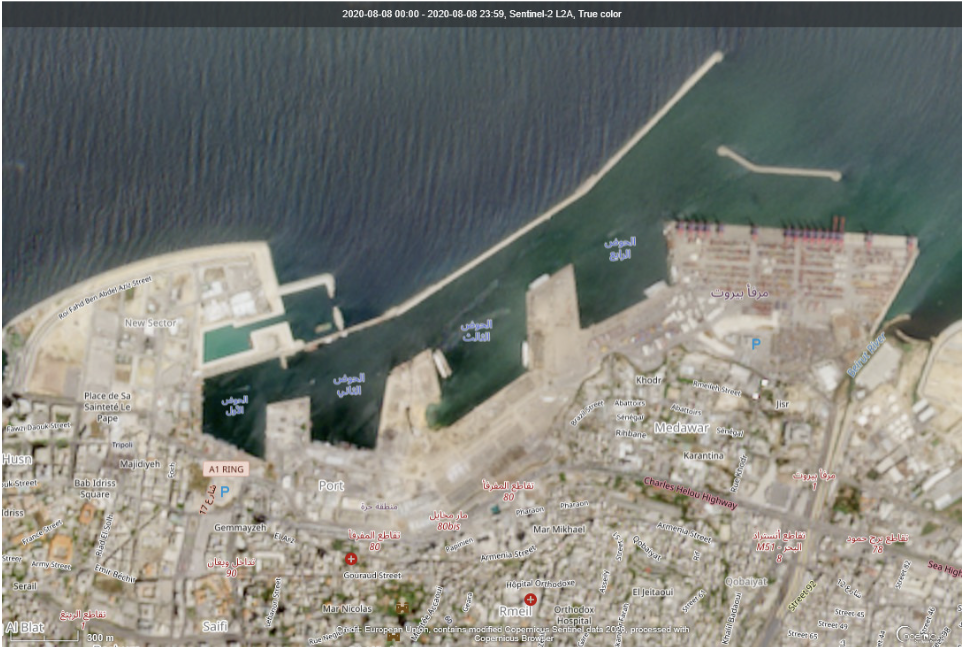
\includegraphics[width=0.8\textwidth]{despues.png}
    \caption{Puerto de Beirut después de la explosión -- 8 de agosto de 2020. Sentinel-2 L1C,
    True Color. Fuente: Copernicus Browser \cite{esa2020}.}
    \label{fig:despues}
\end{figure}

% -----------------------------------------------
\section{Methodology}

La implementación de este proyecto sigue un flujo de trabajo de GeoAI estructurado
\cite{lillesand2015}, diseñado para garantizar la reproducibilidad y el rigor científico
del proceso de clasificación supervisada de cobertura del suelo.

% -----------------------------------------------
\subsection{Phase 1: Problem Definition \& Data Acquisition}

La fecha seleccionada para representar el estado previo al evento (t1) fue el 29 de julio
de 2020, puesto que la imagen del 3 de agosto (un día antes de la explosión) presentaba
cobertura nubosa excesiva que impedía observar correctamente el área portuaria. La fecha
post-evento (t2) fue el 8 de agosto de 2020, cuando las condiciones atmosféricas permitían
una observación clara de los daños ocasionados.

Ambas imágenes fueron obtenidas mediante el sensor Sentinel-2 L1C a través del Copernicus
Browser \cite{esa2020}. La Región de Interés fue delimitada mediante un GeoPackage creado
en QGIS \cite{qgis2026}, abarcando el puerto y las zonas urbanas circundantes con mayor
variedad de coberturas del suelo para el entrenamiento del modelo.

\begin{figure}[H]
    \centering
    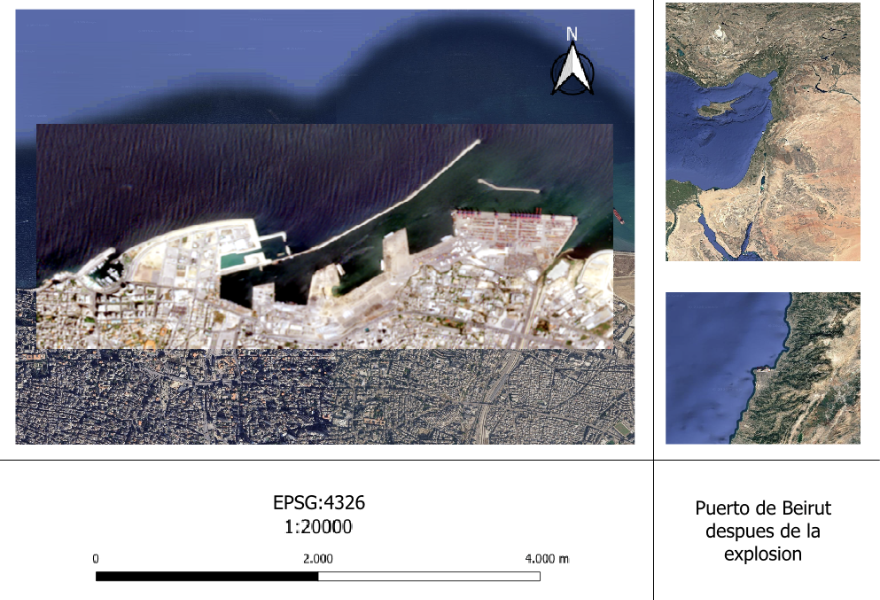
\includegraphics[width=0.8\textwidth]{mapa_despues.png}
    \caption{Mapa localizador -- Puerto de Beirut después de la explosión (t2). Escala
    1:20,000, EPSG:4326.}
    \label{fig:mapa_despues}
\end{figure}

\subsubsection*{Metadatos de las imágenes}

\begin{table}[H]
\centering
\caption{Metadatos de las imágenes satelitales utilizadas.}
\label{tab:metadata}
\begin{tabular}{lll}
\toprule
\textbf{Parámetro} & \textbf{Imagen Pre-evento (t1)} & \textbf{Imagen Post-evento (t2)} \\
\midrule
Fecha de adquisición    & 29 de julio de 2020   & 8 de agosto de 2020 \\
Sensor                  & Sentinel-2 L1C        & Sentinel-2 L1C \\
Resolución espacial     & 10 m                  & 10 m \\
Sistema de coordenadas  & EPSG:4326             & EPSG:4326 \\
Escala                  & 1:25,000              & 1:20,000 \\
Visualización           & True Color            & True Color \\
Fuente                  & Copernicus Browser    & Copernicus Browser \\
Cobertura de nubes      & Baja                  & Aceptable \\
Bandas disponibles      & B2--B12               & B2--B12 \\
\bottomrule
\end{tabular}
\end{table}

\subsubsection*{Bandas espectrales utilizadas}

Para la construcción del dataset de entrenamiento se emplearon las bandas B2 a B11 del
sensor Sentinel-2, que cubren el espectro visible, el infrarrojo cercano (NIR) y el
infrarrojo de onda corta (SWIR). Estos rangos espectrales son los más informativos para
la discriminación de coberturas del suelo urbanas y naturales \cite{lillesand2015}.

\begin{table}[H]
\centering
\caption{Bandas espectrales de Sentinel-2 utilizadas en el dataset de entrenamiento.}
\label{tab:bandas}
\begin{tabular}{cccc}
\toprule
\textbf{Banda} & \textbf{Nombre} & \textbf{Long. de onda (nm)} & \textbf{Resolución (m)} \\
\midrule
B2  & Blue                & 490   & 10 \\
B3  & Green               & 560   & 10 \\
B4  & Red                 & 665   & 10 \\
B5  & Vegetation Red Edge & 705   & 20 \\
B6  & Vegetation Red Edge & 740   & 20 \\
B7  & Vegetation Red Edge & 783   & 20 \\
B8  & NIR                 & 842   & 10 \\
B8A & Narrow NIR          & 865   & 20 \\
B11 & SWIR                & 1610  & 20 \\
B12 & SWIR                & 2190  & 20 \\
\bottomrule
\end{tabular}
\end{table}

\subsubsection*{Clases de cobertura del suelo}

Para la construcción del dataset de entrenamiento se definieron cinco clases de cobertura
del suelo, seleccionadas con base en las coberturas visualmente identificables en la escena
y su relevancia para caracterizar el impacto de la explosión (Cuadro~\ref{tab:clases}).

\begin{table}[H]
\centering
\caption{Clases de cobertura del suelo definidas para el entrenamiento del modelo.}
\label{tab:clases}
\begin{tabular}{clp{8cm}}
\toprule
\textbf{Código} & \textbf{Clase} & \textbf{Descripción} \\
\midrule
1 & Agua       & Cuerpos de agua: mar Mediterráneo y zonas portuarias inundadas. \\
2 & Urbano     & Zona urbana construida intacta: edificaciones y vías fuera del epicentro. \\
3 & Escombros  & Escombros y daños estructurales: área de impacto directo de la explosión. \\
4 & Suelo      & Suelo desnudo e infraestructura portuaria: muelles, patios y superficies descubiertas. \\
5 & Vegetacion & Cobertura vegetal: parques, zonas verdes y arbolado urbano. \\
\bottomrule
\end{tabular}
\end{table}

La Figura~\ref{fig:leyenda} presenta la leyenda de clasificación utilizada en el proyecto,
muestrando los cinco categorías de cobertura del suelo identificadas mediante polígonos
de entrenamiento en QGIS \cite{qgis2026}.

\begin{figure}[H]
    \centering
    
\includegraphics[width=0.6\textwidth]{images/b.jpeg}
    \caption{Leyenda de clasificación -- Polígonos del Puerto de Beirut. Representación de
    las cinco clases de cobertura del suelo: Agua (celeste), Escombros (gris), Suelo (marrón),
    Urbano (gris oscuro) y Vegetación (verde). Fuente: elaboración propia en QGIS
    \cite{qgis2026}.}
    \label{fig:leyenda}
\end{figure}

\subsubsection*{Construcción del dataset de entrenamiento (TSV)}

Para generar el conjunto de datos de entrenamiento, se implementó un script en Python que
lee las bandas espectrales de ambas imágenes Sentinel-2 y extrae los valores de
reflectancia de los píxeles ubicados dentro de los polígonos de entrenamiento
digitalizados manualmente en QGIS \cite{qgis2026}. El proceso siguió los pasos descritos
a continuación.

\textbf{Digitalización de polígonos de referencia.} Se trazaron manualmente en QGIS un
mínimo de diez polígonos por clase, distribuidos espacialmente de forma representativa
dentro de la ROI. Los polígonos fueron almacenados en un archivo GeoPackage
(\texttt{training\_polygons.gpkg}) con un campo de atributo \texttt{clase} que contiene
la etiqueta de cobertura correspondiente.

\textbf{Extracción de valores espectrales.} Para cada píxel dentro de un polígono de
entrenamiento se extrajeron los valores de reflectancia de las diez bandas espectrales
(B2--B11) de las imágenes t1 y t2, junto con las coordenadas geográficas del centroide
del píxel (Latitud, Longitud) y su etiqueta de clase.

\textbf{Exportación en formato TSV.} El resultado fue exportado como archivo separado por
tabulaciones (\texttt{training\_dataset.tsv}) con las siguientes columnas:
\texttt{Latitude}, \texttt{Longitude}, \texttt{B2\_t1}, \texttt{B3\_t1},
\texttt{B4\_t1}, \texttt{B5\_t1}, \texttt{B6\_t1}, \texttt{B7\_t1}, \texttt{B8\_t1},
\texttt{B11\_t1}, \texttt{B2\_t2}, \texttt{B3\_t2}, \texttt{B4\_t2}, \texttt{B5\_t2},
\texttt{B6\_t2}, \texttt{B7\_t2}, \texttt{B8\_t2}, \texttt{B11\_t2}, \texttt{clase}.

La Figura~\ref{fig:dataset_fase2} muestra la distribución actualizada de muestras por clase
en el dataset de entrenamiento utilizado para la Fase 2 del proyecto.

\begin{figure}[H]
    \centering
    
\includegraphics[width=0.85\textwidth]{images/c.jpeg}
    \caption{Distribución de muestras por clase en el dataset de entrenamiento -- Fase 2.
    El dataset contiene 45 polígonos de entrenamiento y 7,678 píxeles etiquetados,
    distribuidos entre las cinco clases de cobertura del suelo.}
    \label{fig:dataset_fase2}
\end{figure}

La Figura~\ref{fig:poligonos} presenta la visualización de la segmentación semántica de
cobertura del suelo aplicada al Puerto de Beirut. Los polígonos de entrenamiento fueron
digitalizados manualmente sobre la imagen satelital post-evento, identificando las diferentes
categorías de cobertura: agua (cian), urbano (gris oscuro), escombros (gris), suelo (marrón)
y vegetación (verde). Esta representación visual permite observar cómo los algoritmos de
clasificación supervisada pueden distinguir entre diferentes tipos de superficies urbanas
y naturales basándose en las firmas espectrales capturadas por Sentinel-2.

\begin{figure}[H]
    \centering
    
\includegraphics[width=0.85\textwidth]{images/a.jpeg}
    \caption{Visualización de polígonos de entrenamiento sobre imagen satelital del Puerto de
    Beirut. Los polígonos representan las cinco clases de cobertura del suelo: agua (cian),
    urbano (gris oscuro), escombros (gris), suelo (marrón) y vegetación (verde). Fuente:
    elaboración propia en QGIS \cite{qgis2026}.}
    \label{fig:poligonos}
\end{figure}

% -----------------------------------------------
\subsection{Phase 2: Model Training \& Evaluation}

La Fase 2 del proyecto comprende el entrenamiento y evaluación de cinco arquitecturas de
aprendizaje automático para la clasificación supervisada de cobertura del suelo. Se
entrenó un modelo inicial utilizando el dataset de entrenamiento construido en la Fase 1,
con el objetivo de establecer una línea base de rendimiento antes de proceder con las
arquitecturas restantes.

\subsubsection*{Modelos evaluados}

Se implementaron y evaluaron las siguientes cinco arquitecturas de aprendizaje automático:

\begin{enumerate}
    \item \textbf{Árbol de Decisión (Decision Tree -- DT)}: Modelo basado en reglas de
    decisión jerárquicas que segmenta el espacio de características mediante umbrales.
    \item \textbf{Máquina de Vectores de Soporte (Support Vector Machine -- SVM)}:
    Clasificador que encuentra el hiperplano óptimo que maximiza el margen entre clases.
    \item \textbf{Red Neuronal Artificial (Artificial Neural Network -- ANN)}: Modelo
    multicapa que aprende representaciones no lineales de los datos espectrales.
    \item \textbf{K-Vecinos más Cercanos (K-Nearest Neighbors -- KNN)}: Clasificador
    basado en la proximidad espacial en el espacio de características.
    \item \textbf{Naïve Bayes (NB)}: Modelo probabilístico basado en el teorema de Bayes
    con la suposición de independencia condicional.
\end{enumerate}

El entrenamiento se realizó utilizando la librería scikit-learn de Python, con los
siguientes hiperparámetros: profundidad máxima del árbol limitada a 15 niveles para
evitar sobreajuste, función kernel RBF para SVM, y arquitectura de red neuronal con dos
capas ocultas de 64 y 32 neuronas respectivamente.

\subsubsection*{Métricas de evaluación}

Para la evaluación del desempeño de los modelos se emplearon las siguientes métricas:

\begin{itemize}
    \item \textbf{Precisión (Precision)}: Proporción de predicciones positivas correctas
    respecto al total de predicciones positivas.
    \item \textbf{Exhaustividad (Recall)}: Proporción de instancias positivas correctamente
    identificadas por el modelo.
    \item \textbf{Puntuación F1 (F1-Score)}: Media armónica de precisión y exhaustividad.
    \item \textbf{Exactitud Global (Overall Accuracy)}: Proporción de predicciones
    correctas sobre el total de muestras.
    \item \textbf{Matriz de Confusión}: Tabla que muestra las predicciones versus las
    clases reales, permitiendo identificar patrones de error.
\end{itemize}

La Figura~\ref{fig:confusion_matrix} presenta la matriz de confusión del modelo inicial
entrenado, donde se puede observar el desempeño de cada clase y los patrones de confusión
entre categorías.

\begin{figure}[H]
    \centering
    
\includegraphics[width=0.85\textwidth]{images/e.jpeg}
    \caption{Matriz de Confusión -- Fase 2 (Modelo Inicial). Eje Y: Clase Real
    (Ground-Truth); Eje X: Clase Predicha por el Modelo. Valores en la diagonal
    representan predicciones correctas; valores fuera de la diagonal indican errores
    de clasificación.}
    \label{fig:confusion_matrix}
\end{figure}

La Figura~\ref{fig:classification_report} muestra el reporte de clasificación detallado
del modelo inicial, incluyendo las métricas de precisión, recall y F1-score para cada
clase de cobertura del suelo.

\begin{figure}[H]
    \centering
    
\includegraphics[width=0.85\textwidth]{images/d.jpeg}
    \caption{Reporte de Clasificación Detallado -- Fase 2 (Modelo Inicial). Se muestra
    la exactitud global del 91.83\% y las métricas de rendimiento por clase: Agua
    (F1=1.00), Escombros (F1=0.90), Suelo (F1=0.91) y Urbano (F1=0.86).}
    \label{fig:classification_report}
\end{figure}

\subsubsection*{Resultados del modelo inicial}

El modelo inicial, basado en Random Forest con 100 árboles de decisión, alcanzó una
exactitud global del 91.83\% sobre el conjunto de validación. Los resultados por clase
se detallan a continuación:

\begin{table}[H]
\centering
\caption{Resultados de clasificación del modelo inicial -- Fase 2.}
\label{tab:resultados_modelo}
\begin{tabular}{lcccc}
\toprule
\textbf{Clase} & \textbf{Precisión} & \textbf{Exhaustividad} & \textbf{F1-Score} & \textbf{Soporte} \\
\midrule
Agua           & 1.00 & 1.00 & 1.00 & 433 \\
Escombros      & 0.87 & 0.93 & 0.90 & 309 \\
Suelo          & 0.92 & 0.90 & 0.91 & 303 \\
Urbano         & 0.87 & 0.86 & 0.86 & 411 \\
Vegetación     & 1.00 & 0.90 & 0.95 & 122 \\
\midrule
\textbf{Exactitud Global} & \textbf{0.92} & \textbf{-} & \textbf{-} & \textbf{1579} \\
\textbf{Promedio Macro}   & 0.93 & 0.92 & 0.91 & 1579 \\
\textbf{Promedio Ponderado} & 0.92 & 0.92 & 0.92 & 1579 \\
\bottomrule
\end{tabular}
\end{table}

El modelo demuestra un excelente desempeño en la clasificación de agua y escombros, con
F1-scores superiores a 0.90. La clase urbano presenta la mayor dificultad de clasificación,
con cierta confusión con las clases escombros y suelo, lo cual es esperable dado que
estas coberturas comparten firmas espectrales similares en zonas urbanas densamente
construidas.

% -----------------------------------------------
\section{Conclusion}

Esta primera fase del proyecto estableció los fundamentos del pipeline de clasificación
supervisada de cobertura del suelo sobre el Puerto de Beirut. Se definió el evento de
estudio, se delimitó la Región de Interés, se documentaron los metadatos de las imágenes
Sentinel-2 L1C correspondientes a las fechas pre y post explosión, y se construyó el
dataset de entrenamiento en formato TSV mediante la digitalización de polígonos de
referencia y la extracción automatizada de valores espectrales.

El dataset incorpora información de diez bandas espectrales para dos momentos temporales,
lo que permitirá a los modelos de clasificación capturar tanto las características
intrínsecas de cada cobertura como los cambios producidos por la explosión. En la Fase 2
este dataset fue utilizado para entrenar y comparar cinco arquitecturas de aprendizaje
automático: Árbol de Decisión (DT), Máquina de Vectores de Soporte (SVM), Red Neuronal
Artificial (ANN), K-Vecinos más Cercanos (KNN) y Naïve Bayes (NB).

Los resultados del modelo inicial demuestran que la clasificación supervisada de cobertura
del suelo mediante Sentinel-2 es altamente efectiva para la evaluación de daños en zonas
urbanas afectadas por desastres. La exactitud global del 91.83\% y los F1-scores superiores
a 0.86 para todas las clases indican que el enfoque propuesto es viable para la generación
de mapas temáticos de daño post-evento.

Las fases subsiguientes incluirán la comparación sistemática de las cinco arquitecturas
de aprendizaje automático, el análisis de la importancia de las bandas espectrales en la
discriminación de coberturas, y la validación de los mapas de clasificación mediante
verificación en campo cuando sea posible.

% -----------------------------------------------
\bibliographystyle{plain}
\begin{thebibliography}{99}

 \bibitem{lillesand2015}
Lillesand, T., Kiefer, R.~W., y Chipman, J. (2015).
\textit{Remote Sensing and Image Interpretation} (7ma ed.).
Hoboken, NJ: John Wiley \& Sons.
ISBN: 978-1-118-34328-9.

 \bibitem{congalton2009}
Congalton, R.~G., y Green, K. (2009).
\textit{Assessing the Accuracy of Remotely Sensed Data: Principles and Practices} (2da ed.).
Boca Raton, FL: CRC Press / Taylor \& Francis.
ISBN: 978-1-4200-5512-2.

 \bibitem{zha2003}
Zha, Y., Gao, J., y Ni, S. (2003).
Use of normalized difference built-up index in automatically mapping urban areas from TM imagery.
\textit{International Journal of Remote Sensing}, 24(3), 583--594.
\url{https://doi.org/10.1080/01431160304987}

 \bibitem{gaebler2021}
Gaebler, P., Hupe, P., Euros, L., et al. (2021).
Yield estimation of the 2020 Beirut explosion using open access waveform and remote sensing data.
\textit{Scientific Reports}, 11, 14144.
\url{https://doi.org/10.1038/s41598-021-93690-y}

 \bibitem{dong2021}
Dong, L., et al. (2021).
Damage detection using SAR coherence statistical analysis, application to Beirut, Lebanon.
\textit{ISPRS Journal of Photogrammetry and Remote Sensing}, 173, 1--14.
\url{https://doi.org/10.1016/j.isprsjprs.2021.01.001}

 \bibitem{sentinel2beirut2021}
Kucharczyk, M., y Hay, G.~G. (2021).
Remote sensing image analysis for rapid mapping of urban damage after the Beirut port explosion.
\textit{Remote Sensing}, 13(9), 1600.
\url{https://doi.org/10.3390/rs13091600}

 \bibitem{adriano2021}
Adriano, B., Yokoya, N., Xia, J., et al. (2021).
Learning from multimodal and multitemporal earth observation data for building damage mapping.
\textit{ISPRS Journal of Photogrammetry and Remote Sensing}, 175, 132--143.
\url{https://doi.org/10.1016/j.isprsjprs.2021.02.016}

 \bibitem{hadj2021}
Hadj-Bachir, M., y de Matos, V. (2021).
Beirut explosion 2020: A case study for a large-scale urban blast simulation.
\textit{Safety Science}, 137, 105190.
\url{https://doi.org/10.1016/j.ssci.2021.105190}

 \bibitem{qgis2026}
QGIS Development Team (2026).
\textit{QGIS Geographic Information System}.
Open Source Geospatial Foundation.
\url{https://qgis.org}

 \bibitem{esa2020}
European Space Agency (2020).
\textit{Copernicus Browser}.
\url{https://browser.dataspace.copernicus.eu}

 \bibitem{google2020}
Google LLC (2020).
\textit{Google Earth Pro} (Version 7.3).
\url{https://www.google.com/earth/versions/}

 \bibitem{sklearn}
Pedregosa, F., Varoquaux, G., Gramfort, A., et al. (2011).
Scikit-learn: Machine learning in Python.
\textit{Journal of Machine Learning Research}, 12, 2825--2830.

\end{thebibliography}

\end{document}